\begin{figure}[t!]

\definecolor{darkorange25512714}{RGB}{255,127,14}
\definecolor{darkslategray38}{RGB}{38,38,38}
\definecolor{lightgray204}{RGB}{204,204,204}
\definecolor{steelblue31119180}{RGB}{31,119,180}

\begin{center}
\footnotesize
\begin{tabular}{cc}
{\color{darkorange25512714}\large \textbf{---}} Point-MAE\,\cite{pang2022pointmae} & {\color{steelblue31119180}\large \textbf{---}}  \textbf{\name{}} (Ours)
 \\
\hspace{2cm}&\hspace{2cm}
\end{tabular}
\end{center}
\vspace{-25px}
\hspace{-17px}

\subcaptionbox{ModelNet40\,\cite{wu2015modelnet40}}{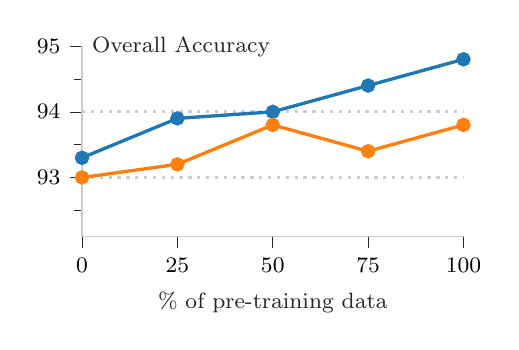
\begin{tikzpicture}

\definecolor{darkorange25512714}{RGB}{255,127,14}
\definecolor{darkslategray38}{RGB}{38,38,38}
\definecolor{lightgray204}{RGB}{204,204,204}
\definecolor{steelblue31119180}{RGB}{31,119,180}

\begin{axis}[
width=0.53\linewidth,height=4cm,
axis x line=bottom,
axis y line=left,
x axis line style={-},
ytick distance=0.5,
minor y tick num=1,
ytick={92, 93, 94, 95},
y axis line style={-},
axis line style={white!80!black},
legend cell align={left},
legend style={
  fill opacity=0.8,
  draw opacity=1,
  text opacity=1,
  at={(0.97,0.03)},
  anchor=south east,
  draw=lightgray204,
  legend image post style={line width =1.0pt}
},
tick align=outside,
xlabel=\textcolor{darkslategray38}{\footnotesize \% of pre-training data},
xmin=0, xmax=100,
xtick={0, 25, 50, 75, 100},
xtick style={color=darkslategray38},
y grid style={lightgray204},
x grid style={lightgray204},
every axis y label/.style={at={(0.001,1.1)},anchor=north west},
ylabel=\textcolor{darkslategray38}{\footnotesize Overall Accuracy},
ymin=92.1, ymax=95.0,
ytick style={color=darkslategray38},
tick label style={font=\footnotesize},
]

\addplot [very thick, dotted, lightgray204]
table {%
0 93
100 93
};

\addplot [very thick, dotted, lightgray204]
table {%
0 94
100 94
};

\addplot [very thick, steelblue31119180, mark=*, mark size=2, mark options={solid}]
table {%
0 93.3
25 93.9
50 94.0
75 94.4
100 94.8
};
\addplot [very thick, darkorange25512714, mark=*, mark size=2, mark options={solid}]
table {%
0 93.0
25 93.2
50 93.8
75 93.4
100 93.8
};

\end{axis}

\end{tikzpicture}}%
\hfill
\subcaptionbox{ScanObjectNN\,\cite{uy2019scanobjectnn}}{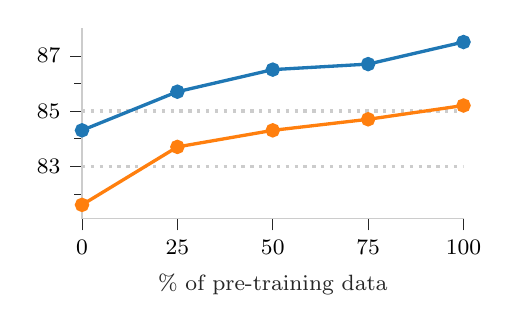
\begin{tikzpicture}

\definecolor{darkorange25512714}{RGB}{255,127,14}
\definecolor{darkslategray38}{RGB}{38,38,38}
\definecolor{lightgray204}{RGB}{204,204,204}
\definecolor{steelblue31119180}{RGB}{31,119,180}

\begin{axis}[
width=0.53\linewidth,height=4cm,
axis x line=bottom,
axis y line=left,
x axis line style={-},
ytick distance=0.5,
minor y tick num=1,
ytick={81, 83, 85, 87},
y axis line style={-},
axis line style={white!80!black},
legend cell align={left},
legend style={
  fill opacity=0.8,
  draw opacity=1,
  text opacity=1,
  at={(0.97,0.03)},
  anchor=south east,
  draw=lightgray204,
  legend image post style={line width =1.0pt}
},
tick align=outside,
xlabel=\textcolor{darkslategray38}{\footnotesize \% of pre-training data},
xmin=0, xmax=100,
xtick={0, 25, 50, 75, 100},
xtick style={color=darkslategray38},
y grid style={lightgray204},
x grid style={lightgray204},
every axis y label/.style={at={(0.001,1.0)},anchor=north west},
ymin=81.1, ymax=88.0,
ytick style={color=darkslategray38},
tick label style={font=\footnotesize},
]

\addplot [very thick, dotted, lightgray204]
table {%
0 83
100 83
};

\addplot [very thick, dotted, lightgray204]
table {%
0 85
100 85
};

\addplot [very thick, steelblue31119180, mark=*, mark size=2, mark options={solid}]
table {%
0 84.3
25 85.7
50 86.5
75 86.7
100 87.5
};
\addplot [very thick, darkorange25512714, mark=*, mark size=2, mark options={solid}]
table {%
0 81.6
25 83.7
50 84.3
75 84.7
100 85.2
};

\end{axis}

\end{tikzpicture}}%

\caption{
\textbf{Pre-training Data Efficiency.}
Irrespective of the quantity of pre-training data used from ShapeNet, \name{} consistently achieves better results than Point-MAE\,\cite{pang2022pointmae} on ModelNet40 (with voting) and the most difficult test split of ScanObjNN.
}
\label{fig:pretraining_data_efficiency}
\vspace{-20pt}
\end{figure}